% Q8：固定副本中的展开图拓扑；所有小面边长均为 1。
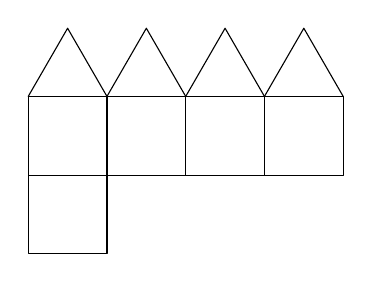
\begin{tikzpicture}[line cap=round,line join=round]
  % 四个侧方形依次相连，底方面连接在最左侧方形下边。
  \draw (0,0) rectangle (1,1);
  \draw (1,0) rectangle (2,1);
  \draw (2,0) rectangle (3,1);
  \draw (3,0) rectangle (4,1);
  \draw (0,-1) rectangle (1,0);
  % 四个等边三角形分别接在侧方形上边。
  \draw (0,1)--(0.5,1.866)--(1,1);
  \draw (1,1)--(1.5,1.866)--(2,1);
  \draw (2,1)--(2.5,1.866)--(3,1);
  \draw (3,1)--(3.5,1.866)--(4,1);
\end{tikzpicture}
